\section{Desarrollo}
	El desarrollo de la práctica consistió en lo siguiente:
	\paragraph{Clases AFD y AFN}
	Ambas clases heredan de un clase padre llamada \textit{Automata}, la cual define los elementos que todo autómata debe tener (Alfabeto, Estados, Función de Transición, Estado Inicial y Estados Finales) y define algunos métodos para que cada tipo de autómata implemente (calcularEstado y validarCadena).\\
	El código de esta clase padre (automata.py) es el siguiente:
	\begin{figure}[H]
		\begin{center}
			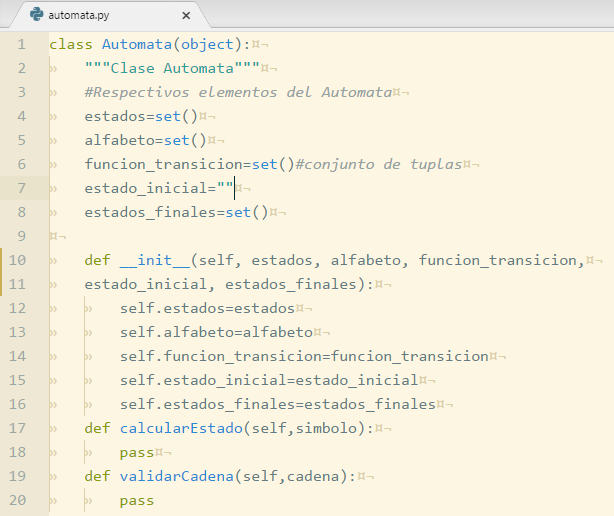
\includegraphics[width=15cm, height=12cm]{img/automata.png}
			\caption{automata.py}
			\label{fig:tablas1}
		\end{center}
	\end{figure}	
	A continuación se muestra el código de la clase AFD la cual actúa como un autómata finito determinista heredando de la clase autómata:\\
	%\lstinputlisting[language=Python, caption=Automata.py]{../afd.py}
	\begin{figure}[H]
		\begin{center}
			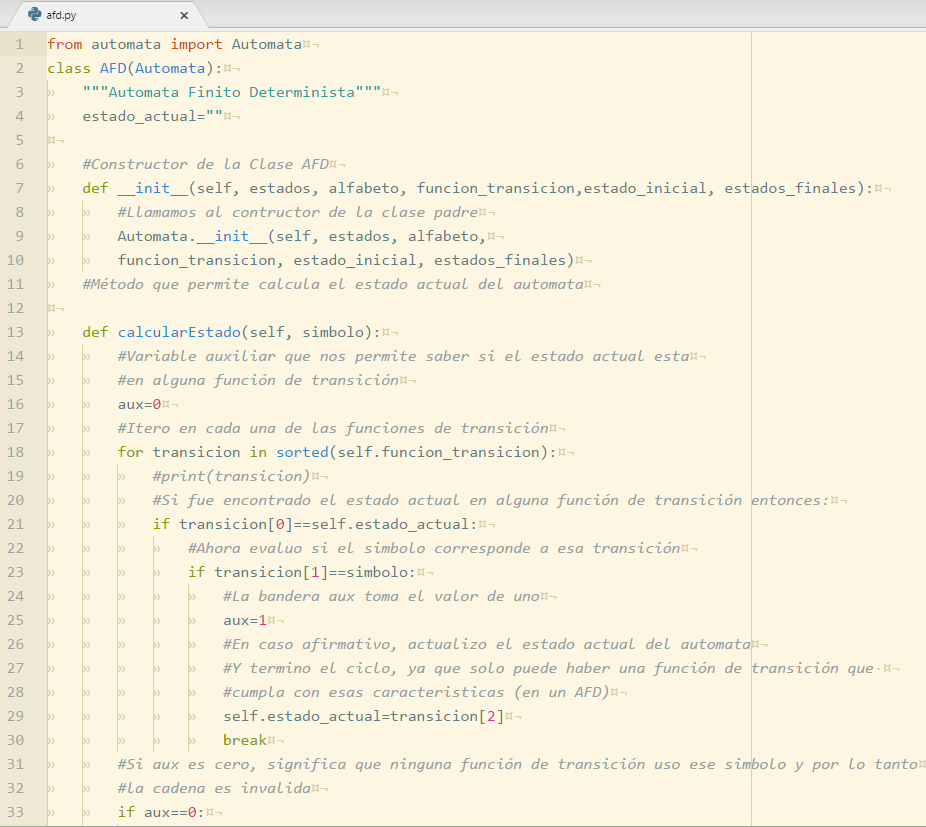
\includegraphics[width=15cm, height=15cm]{img/afd_1.png}
			\caption{afd.py (1)}
			\label{fig:tablas2}
		\end{center}
	\end{figure}
	\begin{figure}[H]
		\begin{center}
			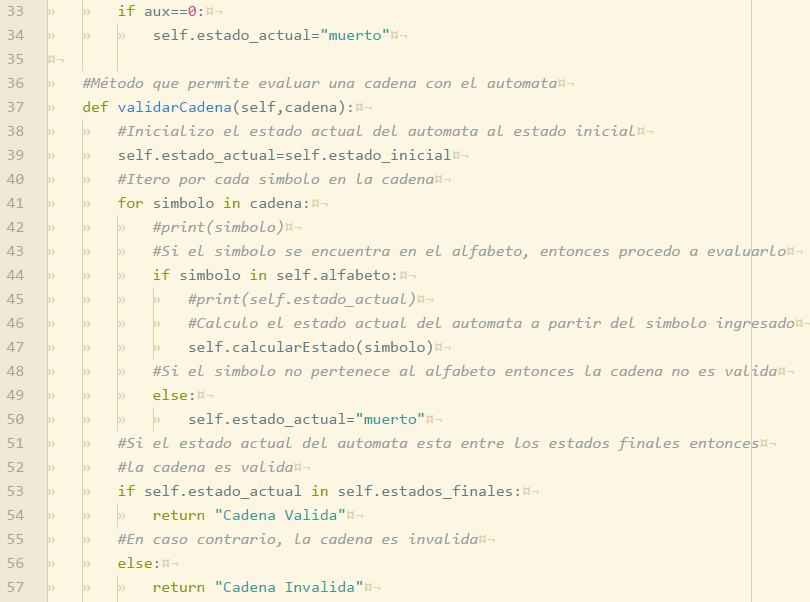
\includegraphics[width=15cm, height=15cm]{img/afd_2.png}
			\caption{afd.py (2)}
			\label{fig:tablas3}
		\end{center}
	\end{figure}
	A continuación se muestra el código de la clase AFND la cual actúa como un autómata finito no determinista (el cual permite las transiciones epsilon), al igual que la clase anterior, hereda de la clase autómata:\\
	\begin{figure}[H]
	\begin{center}
		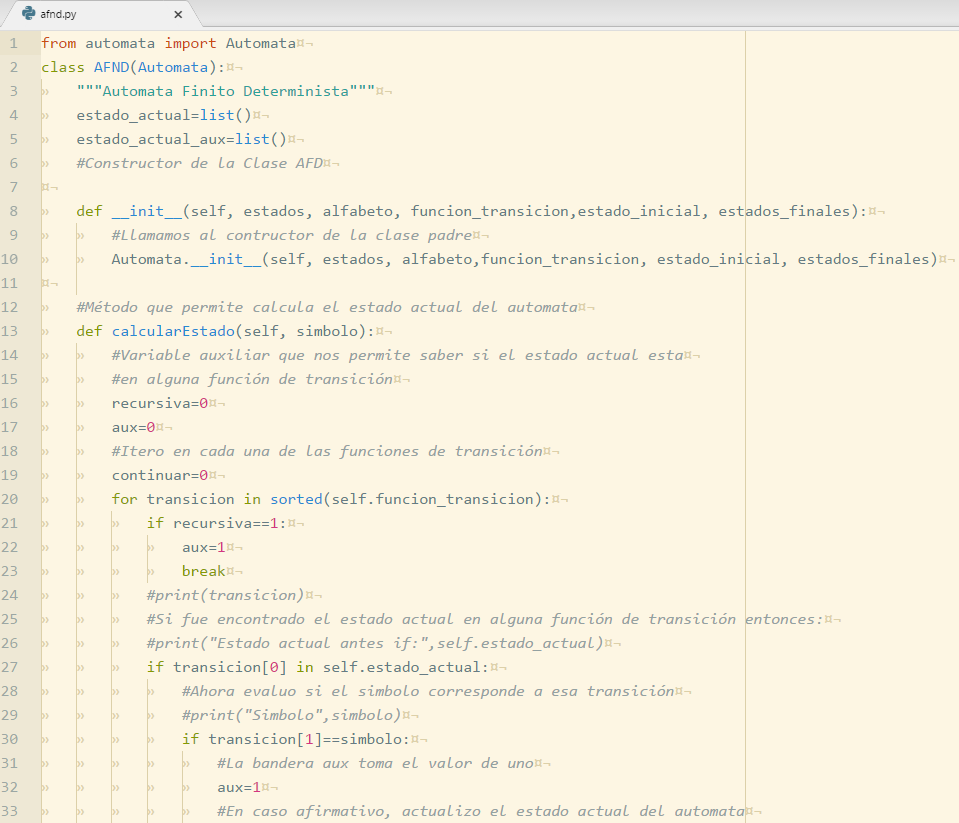
\includegraphics[width=15cm, height=15cm]{img/afnd_1.png}
		\caption{afnd.py (1)}
		\label{fig:tablas4}
	\end{center}
	\end{figure}
	\begin{figure}[H]
		\begin{center}
			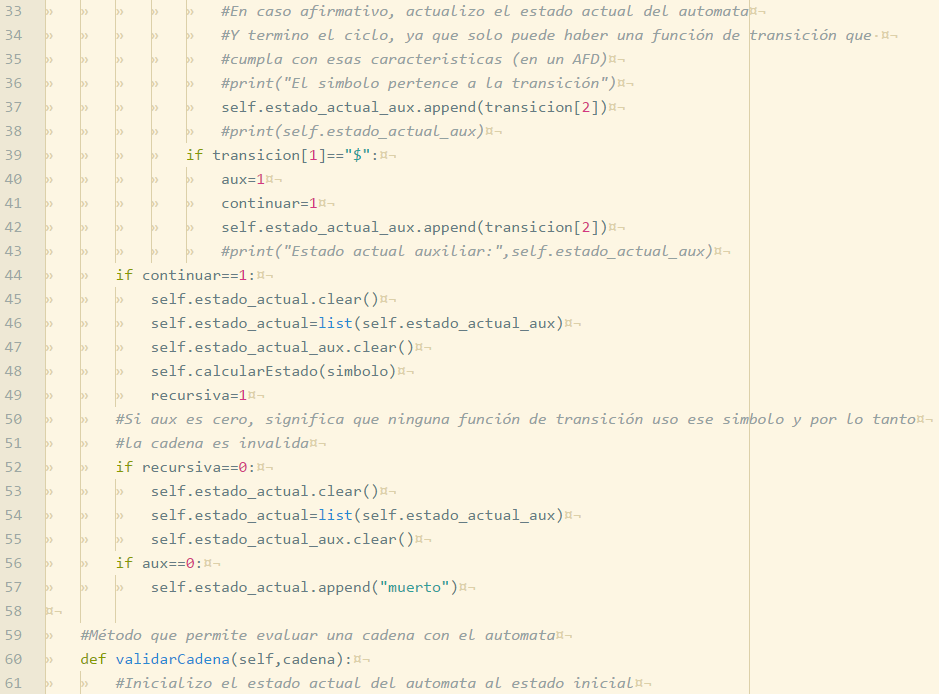
\includegraphics[width=15cm, height=15cm]{img/afnd_2.png}
			\caption{afnd.py (2)}
			\label{fig:tablas5}
		\end{center}
	\end{figure}
	\begin{figure}[H]
		\begin{center}
			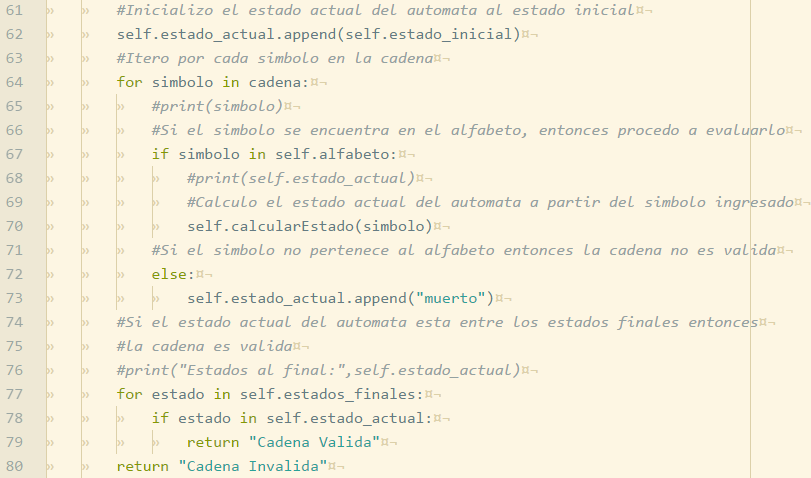
\includegraphics[width=15cm, height=15cm]{img/afnd_3.png}
			\caption{afnd.py (3)}
			\label{fig:tablas6}
		\end{center}
	\end{figure}
	\newpage
	\paragraph{Archivos auxiliares}
	Como se mencionó anteriormente, la información necesaria para la creación de los autómatas es ingresada mediante un archivo el cual es ingresado al momento de ejecutar el programa. El archivo contiene un estructura como la que se indica a continuación:
	\begin{enumerate}
		\item Primer linea: El conjunto de estados del autómata, separados por comas.
		\item Segunda linea: El alfabeto de entrada, igualmente cada símbolo separado por comas.
		\item Tercer linea: función de transición de la siguiente manera: (estado,símbolo,estadoResultado) separadas por guiones.
		\item Cuarta linea: Estado inicial.
		\item Quinta linea: Estados finales o de aceptación separados por comas.
	\end{enumerate}
	Por ende, fue necesario la creación de una clase extra la cual se encargará de manejar el archivo para mandarle la información correspondiente al autómata. El código de este manejador (archivo.py) es el siguiente:
	\begin{figure}[H]
		\begin{center}
			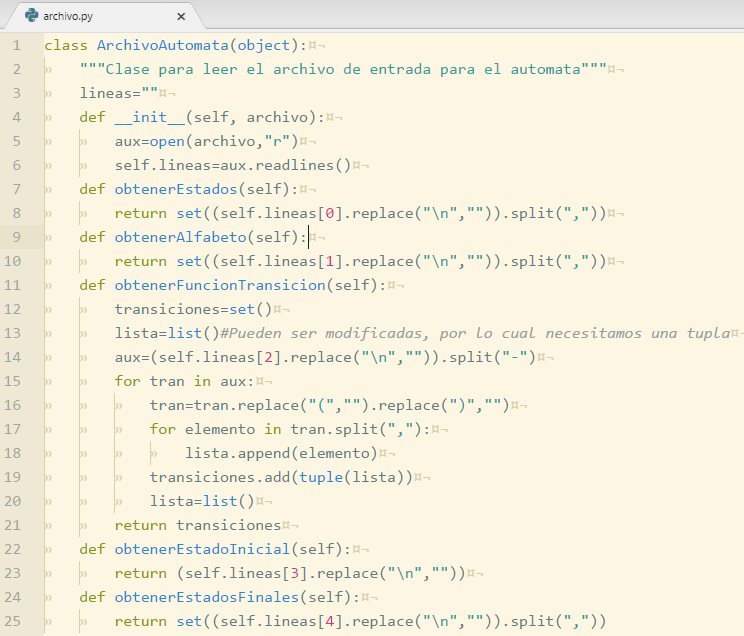
\includegraphics[width=15cm, height=15cm]{img/archivo.png}
			\caption{archivo.py}
			\label{fig:tablas7}
		\end{center}
	\end{figure}